\documentclass{beamer}
\usepackage[utf8]{inputenc}
\usepackage{amsmath}
\usepackage{graphicx}
\usepackage{hyperref}

\title{Sciences humaines, sciences sociales à l'ère numérique : la mise en données et méthodes de modélisation des connaissances}
\author{Stéphane Pouyllau\\ \small{Ingénieur de recherche hors classe CNRS}\\ \small{Professeur attaché à l'université d'Evry-Paris-Saclay}\\ \small{Orcid : 0000-0002-9619-1002}}
\date{Séance du 18 novembre 2024}

\begin{document}

\begin{frame}
    \titlepage
\end{frame}

\begin{frame}{Introduction}
    \begin{itemize}
        \item Objectifs du cours
        \item Importance de la structuration des données
        \item Aperçu des formats CSV, SGBDR, XML (TEI), et RDF
    \end{itemize}
\end{frame}

\begin{frame}{Introduction}
    \begin{figure}
    \centering
    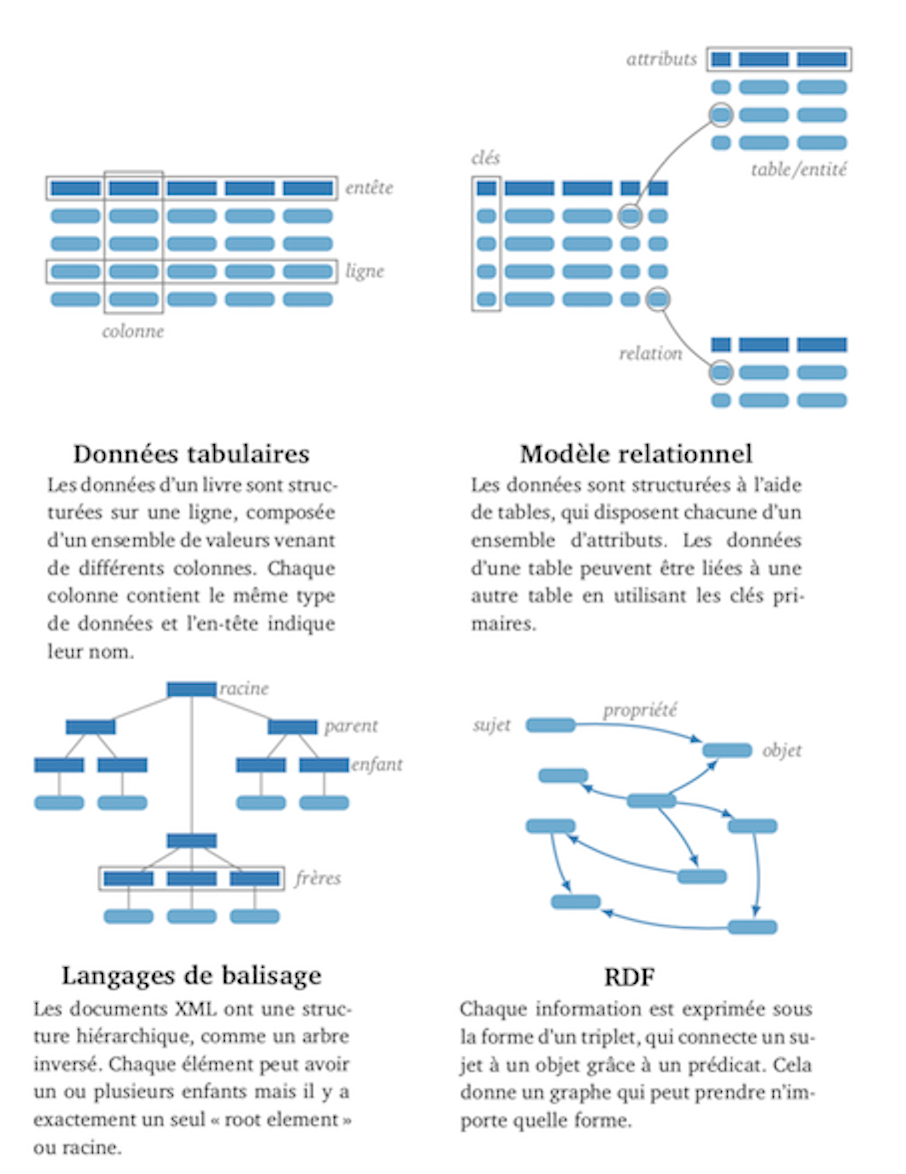
\includegraphics[width=0.5\linewidth]{fig/Setl.png}
    \caption{Seth van Hooland \& al., 2016.}
    \label{fig:enter-label}
\end{figure}
\end{frame}

\begin{frame}{Contexte et applications}
    \begin{itemize}
        \item Utilisations courantes de chaque format
        \item Exemples d'industries et de cas d'utilisation
    \end{itemize}
\end{frame}

\section{CSV (Données Tabulaires)}

\begin{frame}{Introduction à CSV}
    \begin{itemize}
        \item Définition et historique
        \item Structure de base d'un fichier CSV
    \end{itemize}
\end{frame}

\begin{frame}{Syntaxe CSV}
    \begin{itemize}
        \item Séparateurs de colonnes et de lignes
        \item Gestion des valeurs manquantes
    \end{itemize}
\end{frame}

\begin{frame}{Avantages et inconvénients de CSV}
    \begin{itemize}
        \item Simplicité et lisibilité
        \item Limitations en termes de structure et de types de données
    \end{itemize}
\end{frame}

\begin{frame}{Exercice pratique : CSV}
    \begin{itemize}
        \item Créer un fichier CSV
        \item Importer et manipuler des données CSV avec un outil de tableur (Excel, Google Sheets)
    \end{itemize}
\end{frame}

\section{Modèle Relationnel (SGBDR)}

\begin{frame}{Introduction au modèle relationnel}
    \begin{itemize}
        \item Définition et historique
        \item Concepts de base : tables, colonnes, lignes, clés primaires et étrangères
    \end{itemize}
\end{frame}

\begin{frame}{Syntaxe SQL}
    \begin{itemize}
        \item Création de tables
        \item Insertion de données
        \item Requêtes de sélection
    \end{itemize}
\end{frame}

\begin{frame}{Avantages et inconvénients du modèle relationnel}
    \begin{itemize}
        \item Intégrité des données et transactions
        \item Complexité de gestion des relations
    \end{itemize}
\end{frame}

\begin{frame}{Exercice pratique : SGBDR}
    \begin{itemize}
        \item Créer un petit schéma relationnel
        \item Exécuter des requêtes SQL pour manipuler les données
    \end{itemize}
\end{frame}

\section{XML (TEI)}

\begin{frame}{Introduction à XML}
    \begin{itemize}
        \item Définition et historique
        \item Structure de base d'un document XML
    \end{itemize}
\end{frame}

\begin{frame}{Syntaxe XML (TEI)}
    \begin{itemize}
        \item Éléments et attributs
        \item Balises et nœuds
    \end{itemize}
\end{frame}

\begin{frame}{Avantages et inconvénients de XML}
    \begin{itemize}
        \item Flexibilité et extensibilité
        \item Complexité et verbosité
    \end{itemize}
\end{frame}

\begin{frame}{Exercice pratique : XML (TEI)}
    \begin{itemize}
        \item Créer un petit document XML TEI
        \item Valider le document XML avec un outil en ligne
    \end{itemize}
\end{frame}

\section{RDF}

\begin{frame}{Introduction à RDF}
    \begin{itemize}
        \item Définition et historique
        \item Concepts de base : triples, sujets, prédicats, objets
    \end{itemize}
\end{frame}

\begin{frame}{Syntaxe RDF}
    \begin{itemize}
        \item Représentation en XML, Turtle, JSON-LD
    \end{itemize}
\end{frame}

\begin{frame}{Avantages et inconvénients de RDF}
    \begin{itemize}
        \item Flexibilité et interopérabilité
        \item Complexité de gestion des données
    \end{itemize}
\end{frame}

\begin{frame}{Exercice pratique : RDF}
    \begin{itemize}
        \item Créer un petit document RDF
        \item Valider le document RDF avec un outil en ligne
    \end{itemize}
\end{frame}

\section{Conclusion et Q\&A}

\begin{frame}{Résumé des points clés}
    \begin{itemize}
        \item Récapitulatif des formats CSV, SGBDR, XML (TEI), et RDF
        \item Comparaison des avantages et inconvénients
    \end{itemize}
\end{frame}
\end{document}